\documentclass[a4paper,10pt]{article}
%\documentclass[a4paper,10pt]{scrartcl}

\usepackage[utf8]{inputenc}
\usepackage{graphicx}
\usepackage{float}
\usepackage{anysize}

\marginsize{2cm}{2cm}{1cm}{1cm}
\title{Documentación de los programas, tarea 1 elo329.}
\author{Pascal Sigel- Javier Cabezas}
\date{abril-2014}

\pdfinfo{%
  /Title    (Documentación tarea 1 de Programación orientada a objetos UTFSM, 2014 Semestre 1)
  /Author   (Pascal Ernesto Sigel Olivares)
  /Creator  (Pascal Ernesto Sigel Olivares)
  /Producer ()
  /Subject  ()
  /Keywords (Programación orientada a objetos, POO, UTFSM, elo329, Simulación de experimentos simples, simulación)
}

\begin{document}
\maketitle
\newpage
\section{Introducción:}


En el presente documento se explicará cada uno de los programas los cuales están cada uno en su carpeta personal llamada etapa(n) donde n 
es un número. El proyecto está separado en varias etapas, desde la número 1 hasta la número 5 y cada etapa agrega alguna característica a 
la anterior.\newline

El proyecto en sí es un simulador de interacciones físicas como, por ejemplo, el choque de dos bolas, una bola junto con un resorte 
o un bloque con rose con bolas y resortes en cualquier disposición deseada.\newline

En la próxima sección se mostrarán algunos detalles importantes de el programa etapa1, que consta de dos bolas una en resposo y la otra en 
movimiento que chocan con choque elástico.

\section{Etapa 1}

El programa etapa 1 es la primera versión de este simulador el cual simula la interacción de dos bolas que chocan. 
En este programa se crea la primera versión del simulador con las clases PhysicsLab,MyWorld, PhysicsElement y Ball. Se hará
una descripción de cada una de estas clases.\newline


\subsection{Clases e interfaces:}


\subsubsection{Clase PhysicsLab:}


La clase PhysicsLab es la clase main del proyecto, esta clase manipula el objeto de tipo MyWorld creándolo y dándole los elementos que
interaccionarán en este ``mundo'' simulado.\newline

\subsubsection{Clase MyWorld:}


Esta clase es la que maneja la interacción entre los elementos del mundo simulado, el método principal de esta clase es el método \textbf{simulate}
el cual comienza la simulación. En la función \textbf{simulate} 
se requiere que cada elemento físico (PhysycsElement) sea capaz de calcular su próximo estado.\newline

\subsubsection{PhysicsElement:}


Los elementos físicos son una clase abstracta de la cual nacen los elementos como bolas, resores, bloques y cualquier otro elemento físico.\newline

\subsubsection{Ball:}


Esta clase se extiende (desciende) de la clase PhysicsElement y representa una bola la cual tiene masa, velocidad y posicion. En esta clase 
se calcula el próximo estado.\newline


\subsection{Experimento y resultados:}

Lease el archivo README para ejecutar el programa.\newline

El caso ha simular puede ser representado con la siguiente figura:

\begin{figure}[H]
 \centering
 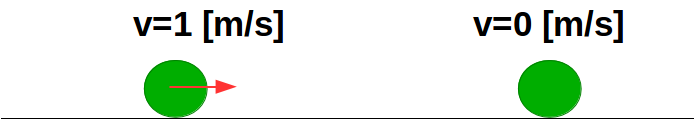
\includegraphics[scale=0.3]{./FigureA.png}
 \caption{Simulación realizada en etapa 1, en la simulación la posición inicial de la bola con velocidad es x=1[mts] y la otra es en x=2.56[mts] ambos con radio 0.1 [mts].}
  \label{etapa1.1}
\end{figure}


Se ha simulado la situación descrita en la figura \ref{etapa1.1}, o sea el choque elástico entre dos
bolas, con la simulación se obtuvieron el siguiente gráfico.

\begin{figure}[H]
 \centering
 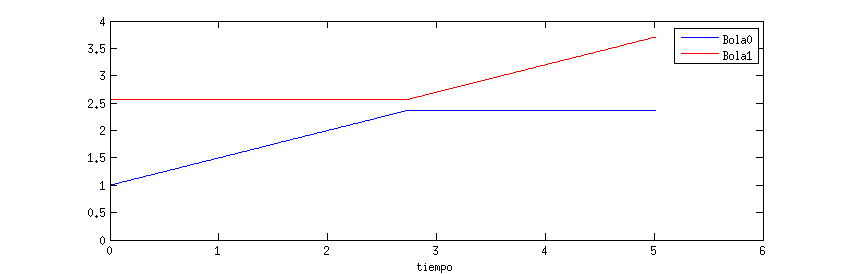
\includegraphics[scale=0.5]{./simulacion_etapa1.png}
 \caption{Resultados simulación etapa 1, Bola 0: bola inicialmente en movimiento y Bola 1: vola inicialmente en reposo.}
  \label{etapa1.2}
\end{figure}

Como se observa en el gráfico de la figura \ref{etapa1.2} cuando la bola 0 colisiona con la bola 1 (a 0.2 mts de distancia dado sus radios) 
la bola 1 obtiene todo el movimiento como se esperaría de un choque elástico de dos masas iguales y una en reposo.\newline

\subsection{Problemas que ocurrieron:}

\subsubsection{Problema con formatos:}


Por defecto Java usa el formato de numeros flotantes con coma ``,'' pero software como matlab usan el formato flotante con punto ``.''
Por lo que en vez de usar \textbf{System.out.print()} se usó \textbf{System.out.format(Locale.US, ... )}.\newline


\subsubsection{Elección de delta t:}


Si el delta t es muy grande entonces el computo de colisión no alcanza a ocurrir cuando una de las bolas ya atravezó a la otra, por ejemplo
si la velocidad de la bola 0 fueran 100 [mts/s] y el delta t es 1[s] entonces en el siguiente cómputo la bola 0 a avanzado 100 mts y probablemente
atravezó a la bola 1 sin la ocurrencia de colisión.\newline

Con esto se da por terminada la primera etapa y se sigue con la siguiente etapa en la cual se agrega el elemento físico resorte.\newline

\section{Etapa 2}

Es la segunda etapa del programa, en esta etapa se agrega los elementos físicos tipo resorte (Spring) con la clase Spring.java.

\subsection{Clases e interfaces:}

\subsubsection{Clase Spring:}

La clase spring extiende de la clase PhysicsElement y representa un resorte, la implementación del resorte consta de asociar cada extremo a 
una bola y sabiendo la posición de las bolas de cada uno de sus extremos se puede calcular la fuerza que este resorte efectúa ha cada
uno de sus extremos.\newline

\subsection{Experimento y resultados:}

Lease el archivo README para ejecutar el programa.\newline

El caso ha simular puede ser representado con la siguiente figura:

\begin{figure}[H]
 \centering
 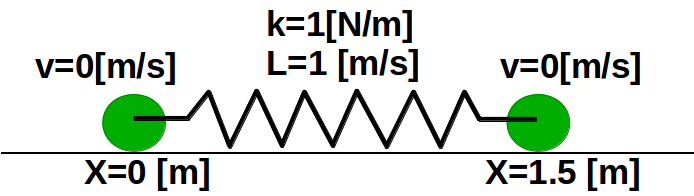
\includegraphics[scale=0.3]{./FigureB.png}
 \caption{Simulación realizada en etapa 2, en la simulación ambas bolas comienzan en reposo una en x=0[mts] y la otra es en x=1.5[mts]
 ambos con radio 0.1 [mts], el resorte efectúa fuerzas según la ley de hooke sobre ambas bolas con stifness = 1 y largo natural 1.}
  \label{etapa2.1}
\end{figure}

Se ha simulado la situación descrita en la figura \ref{etapa2.1}. Con la simulación se obtuvo el siguiente gráfico.

\begin{figure}[H]
 \centering
 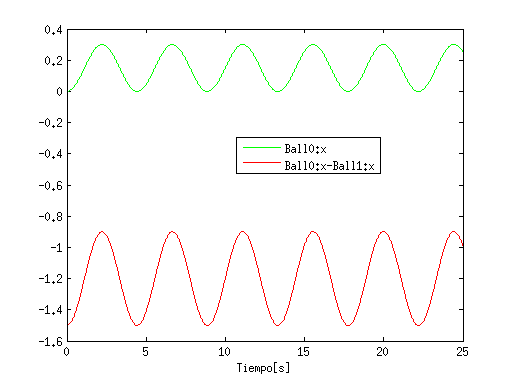
\includegraphics[scale=0.5]{./simulacion_etapa2.png}
 \caption{Resultados simulación etapa 2, en el gráfico se muestran dos diferentes datos en uno la posición de la bola que está inicialmente
 situada en 0 y la otra es la diferencia entre las bolas.}
  \label{etapa2.2}
\end{figure}

  Se observa un comportamiento deseado: ambas bolas oscilan y además su distancia también oscila demostrando que el resorte se contrae y 
  se acercan  y se expande como se esperaría de la situación ideal presentada.\newline
  
\section{Etapa 3:}
 
 En esta etapa se agrega la opción de que el resorte tenga un extremo fijo que representa el objeto FixedHook (FixedHook.java).\newline
 
 
 Desde esta etapa y en adelante se hacen cambios significativos a la estructura del código trabajando de forma más genérica que antes
 usando las interfaces Computable, Collidable, SpringAttachable para los objetos que computan sus estados, colisionan y pueden engancharse
 a un resorte respectivamente. Lo que se busca es que el código sea más fácil de extrapolar a nuevas ideas por lo que la mayor parte de
 las funciones tienen como entrada simplemente un objeto físico y luego si la función es parte de una de las interfaces entonces usa una 
 referencia a la interfaz para calcular todos los computos necesarios.\newline
 
 
 Respecto a las clases, la estructura general de ellas quedan intactas simplemente fueron cambiados los métodos y cosas menores así que se 
 describirán sólo las interfaces nuevas y las clases nuevas.\newline
 
 
\subsection{Clases e interfaces:}
\subsubsection{Clase FixedHook:}


 La clase FixedHook extiende de PhysicsElement e implementa las interfaces Collidable y SpringAttachable sólo no implementa la interfaz Computable
 dado que no cambia de posición en el tiempo. La implementación de esta clase emula la de una bola (Ball.java).\newline
 
 \subsubsection{Interfaz Computable:}
 
 
  No todos los objetos físicos necesariamente tienen que ser capaces de calcular su próximo estado, por ejemplo FixedHook no cambia de posición,
  o lo mismo ocurre con un resorte dado que sus principales valores dependen de las bolas que tiene a sus extremos otro tipo de objetos 
  como las bolas o como se verá más adelante los bloques sí deben computar su próximo estado.\newline
 
 
 \subsubsection{Interfaz Collidable:}
  
  
  Todos los objetos debieran ser colisionables, pero la implementación de esto sería engorrosa debido que algunos objetos jamas van a colisionar
  como es el ejemplo de los resortes, luego para no tener que implementar métodos vacíos se prefiere crear esta interfaz.\newline
  
  \subsection{Experimento y resultados:}
  
  Lease el archivo README para ejecutar el programa.\newline
  
 El caso ha simular puede ser representado con la siguiente figura:
 
 \begin{figure}[H]
 \centering
 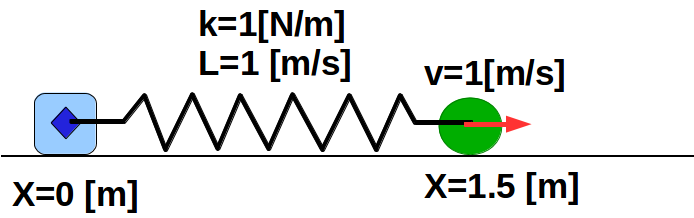
\includegraphics[scale=0.3]{./FigureC.png}
 \caption{Simulación realizada en etapa 3, en la simulación el FixedHook está en x=0.0[mts] y la bola en x=1.5[mts] 
 la bola de radio 0.1 [mts], el resorte efectúa fuerzas según la ley de hooke con stifness = 1 y largo natural 1.}
  \label{etapa3.1}
\end{figure}

  Se ha simulado la situación descrita en la figura \ref{etapa3.1}. Con la simulación se obtuvo el siguiente gráfico.

\begin{figure}[H]
 \centering
 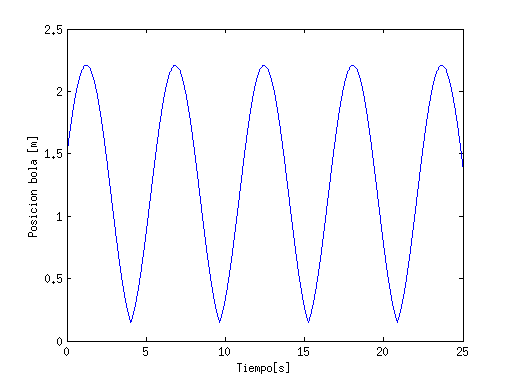
\includegraphics[scale=0.5]{./simulacion_etapa3.png}
 \caption{Resultados simulación etapa 3, en el gráfico se muestra la posición de la bola en el tiempo.}
  \label{etapa3.2}
\end{figure}

\section{Etapa 4:}
  Esta etapa no es más que la demostración de la funcionalidad de la etapa 3.
  
\subsection{Experimento y resultados:}

 El caso ha simular puede ser representado con la siguiente figura:

Lease el archivo README para ejecutar el programa.\newline
  
 El caso ha simular puede ser representado con la siguiente figura:
  
   \begin{figure}[H]
 \centering
 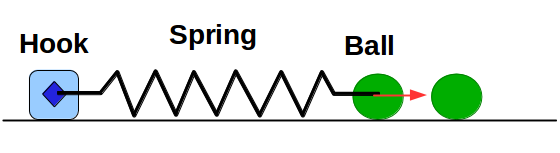
\includegraphics[scale=0.3]{./Figure1.png}
 \caption{Simulación realizada en etapa 4, en la simulación el FixedHook está en x=0.0[mts] y la bola en x=1.5[mts], la bola libre
 se posiciona en x=1.8[mts]
 ambas bolas de radio 0.1 [mts], el resorte efectúa fuerzas según la ley de hooke con stifness = 1 y largo natural 1.}
  \label{etapa4.1}
\end{figure}


Se ha simulado la situación descrita en la figura \ref{etapa4.1}. Con la simulación se obtuvo el siguiente gráfico.


\begin{figure}[H]
 \centering
 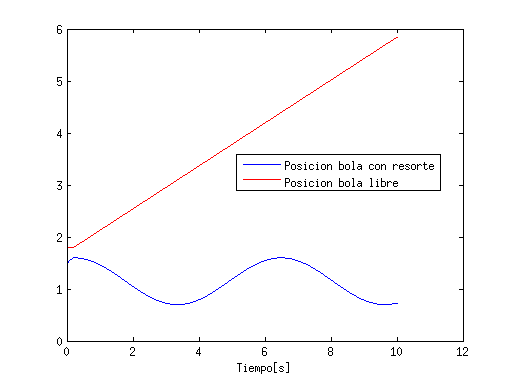
\includegraphics[scale=0.5]{./simulacion_etapa4.png}
 \caption{Resultados simulación etapa 4, en el gráfico se muestran la posición de la bola que está atada al resorte y la de la bola libre respecto al tiempo.}
  \label{etapa3.2}
\end{figure}

\end{document}